% !TeX root = ../main.tex
\documentclass[./../main.tex]{subfiles}

\begin{document}

Bài kiểm thử sẽ được đánh giá thành hai bài kiểm thử
\begin{enumerate}
	\item Bài kiểm thử tự phát triển được em tự triển khai với mục đích đánh
	      giá các chức năng được phát triển có thể xác minh và khai các lỗ hổng
	      đã được phát triển hay không.
	\item Bài kiểm thử thực tế thứ hai đánh giá trên môi trường là dự án
	      DVWA được OWASP phát triển cho mục đích học tập về an ninh ứng dụng Web.
\end{enumerate}

\section{Thử nghiệm trên môi trường tự phát triển}

Để đánh giá được lỗ hổng, em tự xây dựng một bài kiểm tra cho công cụ kiểm
thử tự động ở trên. Để tập trung vào lỗ hổng đã xây dựng, em chỉ xây dựng
các lỗ hổng cho công cụ mình có thể khai thác. Các lỗ hổng khác sẽ nằm
ngoài phạm vi đánh giá của bài thử nghiệm này.

\subsection{Về môi trường thử nghiệm}

\begin{description}
	\item[Ngôn ngữ] PHP 7.2 và Python.

	\item [Cơ sở dữ liệu] MySql 5.7.38

	\item [Môi trường triển khai] Docker.
\end{description}

\subsection{Về các chức năng và lỗ hổng}

\subsubsection{Tìm kiếm người dùng}

\begin{description}
	\item[Mô tả] Chức năng cho phép tìm kiếm người dùng khi nhập đúng
	      thông tin gồm username và password.
	\item [Loại lỗ hổng] SQL Injection
\end{description}

\subsubsection{Xem thông tin Domain}

\begin{description}
	\item[Mô tả] Chức năng cho sử dụng câu lệnh `host` của hệ thống để đưa ra thông tin về ip, tên miền của website được nhập vào.
	\item[Loại lỗ hổng] Command Injection.
\end{description}

\subsubsection{Biểu diễn trang}

\begin{description}
	\item[Mô tả] trang để biểu diễn một đoạn từ file khác được bằng cách
	      include file vào nhưng cho phép người dùng điều chính tên trang.
	\item[Loại lỗ hổng] Path Traversal, Local File Inclusion, Remote
	      File Inclusion.
\end{description}

\subsubsection{Xin chào}

\begin{description}
	\item[Mô tả] Một trang cho phép nhập tên người dùng để in ra sử dụng một template engine.
	\item[Loại lỗ hổng] Server Side Template Injection.
\end{description}


\section{Đánh giá trên môi trường tự phát triển}

Kết quả việc tự động kiểm thử và sử dụng tính năng tự xác minh lỗi
hổng được phát triển \ref{fig:result_test}.

Mặc dù Naf không quét đủ được các lỗ hổng so với Invicti nhưng đã khai thác tốt hơn với lỗ hổng Server Side Template Injection.

\begin{table}[H]
	\begin{tabular}{|l|l|l|l|}
		\hline
		\textbf{Lỗ hổng}               & \textbf{Số lượng} & \textbf{Đã xác minh?} & \textbf{Khai thác?} \\ \hline
		Server Side Template Injection & 0                 &                       & Có                  \\ \hline
		OS Command Injection           & 1                 & Có                    & Có                  \\ \hline
		SQL Injection                  & 2                 & Có                    & Có                  \\ \hline
		Remote File Inclusion          & 1                 & Có                    & Có                  \\ \hline
		Local File Inclusion           & 1                 & Có                    & Có                  \\ \hline
	\end{tabular}
	\caption{Kết quả đánh thử nghiệm của NAF trên môi trường tự phát triển}
\end{table}

\begin{figure}[h!]
	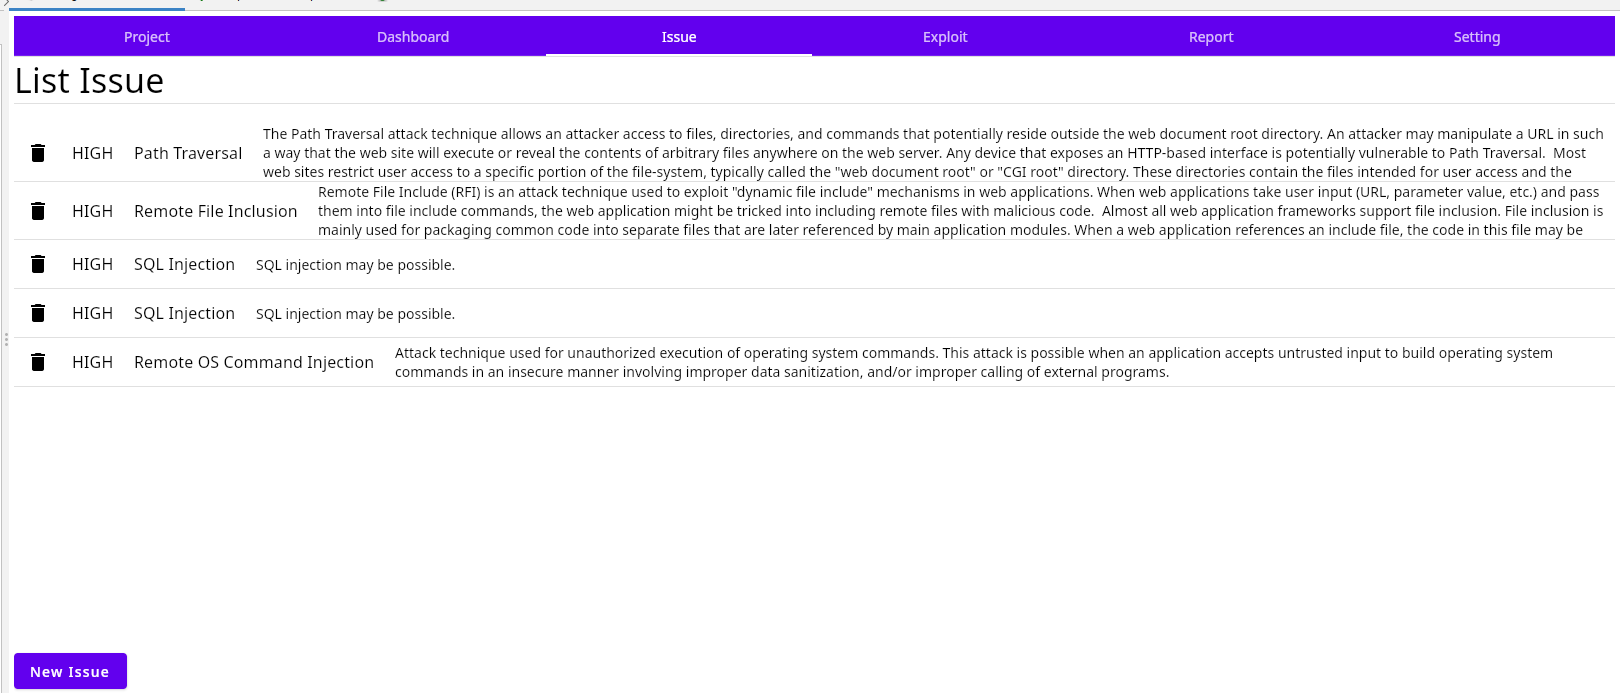
\includegraphics[width=\linewidth]{./images/result_test.png}
	\caption{Kết quả đánh thử nghiệm của NAF trên môi trường tự phát triển}
	\label{fig:result_test}
\end{figure}

Đồng thời đánh giá với Invicti (Nesparker) 5.8.1 là một công cụ thương mại,
em được kết quả như sau.
\begin{table}[H]
	\begin{tabular}{|l|l|l|l|}
		\hline
		\textbf{Lỗ hổng}               & \textbf{Số lượng} & \textbf{Đã xác minh?} & \textbf{Khai thác?} \\ \hline
		Server Side Template Injection & 1                 & Không                 & Không               \\ \hline
		OS Command Injection           & 1                 & Có                    & Có                  \\ \hline
		SQL Injection                  & 2                 & Có                    & Có                  \\ \hline
		Remote File Inclusion          & 1                 & Có                    & Có                  \\ \hline
		Local File Inclusion           & 1                 & Có                    & Có                  \\ \hline
	\end{tabular}
	\caption{Kết quả đánh thử nghiệm của Nesparker trên môi trường tự phát triển}

\end{table}

\section{Thử nghiệm trên dự án DVWA}

Tương tự bài đánh giá trên, bài đánh giá này sẽ chỉ tập trung vào các lỗ
hổng mà công cụ NAF đã được xây dựng để xác minh, các lỗ hổng khác sẽ nắm
ngoài phạm vi đánh giá của bài thử nghiệm này.

\subsection{Về môi trường thử nghiệm}

Môi trường triển khai: DVWA 1.9 đựa trên image vulnerables/web-dvwa.

\section{Đánh giá trên dự án DVWA}



\end{document}

